\newcommand{\imsize}{1.25cm}

\begin{figure*}[ht]
    \centering
    \begin{small}
    \begin{sc}
    \begin{tikzpicture}[node distance=.1cm, auto]
    
    \tikzstyle{header} = [text centered]
    \tikzstyle{pict} = [inner sep=0px]
    \tikzstyle{inputoutput} = [rectangle, rounded corners,text centered, draw=black]
    \tikzstyle{arrow} = [thick,->,-{Latex[scale=1]}]
    \tikzstyle{net} = [rectangle, rounded corners, minimum width=0cm, minimum height=1.8cm,text centered, draw=black, fill=blue!20, shape border rotate=270, trapezium angle=80]
    

    \node [pict, label={[align=right,rotate=90,label distance=-.5cm,yshift=.15cm]left:50\%}] (scale1) {\includesvg[width=\imsize]{figures/elasticities/scale/zoom0.5.svg}};
    \node [pict, below=of scale1, label={[align=right,rotate=90,label distance=-.5cm,yshift=.15cm]left:75\%}] (scale2) {\includesvg[width=\imsize]{figures/elasticities/scale/zoom0.75.svg}};
    \node [pict, below=of scale2, label={[align=right,rotate=90,label distance=-.5cm,yshift=.15cm]left:150\%}] (scale3) {\includesvg[width=\imsize]{figures/elasticities/scale/zoom1.5.svg}};

    \node [header, above=of scale1] (headerscale) {\makecell[c]{Scale}};

    \node [pict, right=.5cm of scale1, label={[align=right,rotate=90,label distance=-.5cm,yshift=.15cm]left:12.5\%}] (pos1) {\includesvg[width=\imsize]{figures/elasticities/position/shake12.5.svg}};
    \node [pict, label={[align=right,rotate=90,label distance=-.5cm,yshift=.15cm]left:25\%}] at (scale2 -| pos1) (pos2) {\includesvg[width=\imsize]{figures/elasticities/position/shake25.svg}};
    \node [pict, label={[align=right,rotate=90,label distance=-.5cm,yshift=.15cm]left:50\%}] at (scale3 -| pos1) (pos3) {\includesvg[width=\imsize]{figures/elasticities/position/shake50.svg}};

    \node [header] at (headerscale -| pos1) (headerposition) {\makecell[c]{Position}};

    \node [pict, right=.5cm of pos1, label={[align=right,rotate=90,label distance=-.5cm,yshift=.15cm]left:20\%}] (drop1) {\includesvg[width=\imsize]{figures/elasticities/dropout/drop20.svg}};
    \node [pict, label={[align=right,rotate=90,label distance=-.5cm,yshift=.15cm]left:40\%}] at (scale2 -| drop1) (drop2) {\includesvg[width=\imsize]{figures/elasticities/dropout/drop40.svg}};
    \node [pict, label={[align=right,rotate=90,label distance=-.5cm,yshift=.15cm]left:80\%}] at (scale3 -| drop1) (drop3) {\includesvg[width=\imsize]{figures/elasticities/dropout/drop80.svg}};

    \node [header] at (headerscale -| drop1) (headerdropout) {\makecell[c]{Missing data}};

    \node[draw,label=above:Perturbations,fit=(headerscale) (scale3) (scale3) (drop3), fit margins={left=.2cm,right=.2cm,bottom=.1cm,top=0cm}, rounded corners] (augs) {};

        
    \node [inputoutput, left=.5cm of augs] (input) {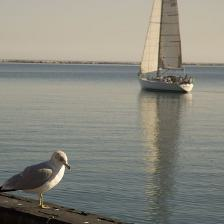
\includegraphics[width=1.5cm]{figures/teaser/0.jpg}};
    \node [header] at (headerscale -| input) (headerinput) {\makecell[c]{Input\\image\\($I$)}};

    \node [inputoutput, right=.5cm of augs] (output) {\makecell[c]{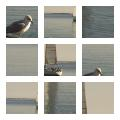
\includegraphics[width=2cm]{figures/teaser/4.jpg}\\$+ \text{pos.enc.}$}};    
    \node [header] at (headerscale -| output) (headeroutput) {\makecell[c]{Patches\\($P'$)}};

    \draw [arrow] (input) -- (augs);
    \draw [arrow] (augs) -- (output);

    \node [net, right=.5cm of output] (vit) {\makecell[c]{Vision\\Transformer}};
    \draw [arrow] (output) -- (vit);
    \node [inputoutput, right=.5cm of vit] (pres) {$\pred(I)$};
    \draw [arrow] (vit) -- (pres);
        
    \end{tikzpicture}
    \end{sc}
    \end{small}
    \caption{\textbf{Evaluation protocol:} To analyze scale, position, and missing data elasticity we introduce three types of perturbations that are applied separately to each patch from the sampling grid.}
    \label{fig:eval-protocol}
\end{figure*}